\documentclass{beamer}
\usetheme{Madrid}
\usepackage{multicol}
\definecolor{ReedRed}{RGB}{167, 14, 22} %Reed Red (primary)
\usecolortheme[named=ReedRed]{structure}
\useoutertheme{miniframes}
\useinnertheme{circles}
\usepackage{soul}

\usepackage{listings}


\usepackage{multicol}
\usepackage{tikz}
\usetikzlibrary{snakes}
\usepackage{rotating}

\usepackage[style=apa,backend=biber,citestyle=numeric]{biblatex}
\addbibresource{../refs.bib}

\title{Bayesian Neural Networks}
\author{
	Ava, Conor, \& Taylor
}
\logo{
	
\includegraphics[width=1cm]{../Images/reed-logo.png}
}
\institute{Reed College}
\setbeamertemplate{navigation symbols}{} % Remove nav bar



\begin{document}
	\section{Intro}
	
\begin{frame}[plain]
    \maketitle
\end{frame}



\begin{frame}{A Brief History}
	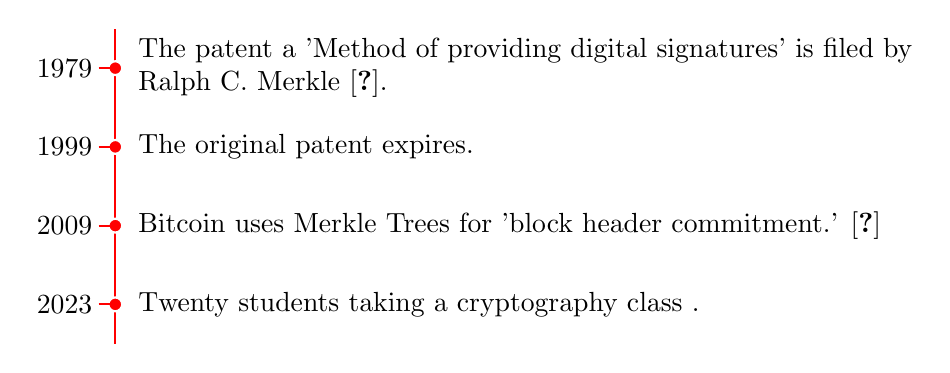
\begin{tikzpicture}[scale=0.5,every node/.style={outer sep=5pt}]
		%Notation: {year, the title of the event}
		%NOTE! Everyting is zero-based
		\def\ourInfo{{
				{"1979"," The patent a 'Method of providing digital signatures' is filed by \\ Ralph C. Merkle  \cite{merkle-patent}."},
				{"1999","The  original patent expires."},
				{"2009","Bitcoin uses Merkle Trees for 'block header commitment.' \cite{friedenbach_alm_2017}"},			
				{"2023","Twenty students taking a cryptography class ."},
		}}
		\pgfmathsetmacro{\length}{3}% Zero based.
		
		% Loop through the array containing all events.
		\foreach \i in {0, ..., \length}{
			\pgfmathsetmacro{\year}{\ourInfo[\i][0]}% Get the left cell (year)
			\pgfmathsetmacro{\eventName}{\ourInfo[\i][1]}% Get the right cell (event name)
			\draw[thick,red] (0,-2*\i-2)--(0,-2*\i);% Draw vertical line
			\ifnum \i=0 % Should be in red text
			\draw(0,-2*\i-1) node[black, right, align = left]{\eventName};% Display the event name
			\draw(0,-2*\i-1) node[black, left] {\year};
			\else % Should be in black text
			\draw(0,-2*\i-1) node[right, black]{\eventName};% Display the event name
			\draw(0,-2*\i-1) node[left] {\year};% Display the year
			\fi
		}
		% Draw the bullet with the dash
		\foreach \i in {0, ..., \length}{
			\filldraw[draw = white, fill = red,thick] (0,-2*\i-1) circle (5pt);
			\draw[thick,red] (-12pt,-2*\i-1)--(0,-2*\i-1);
		}
	\end{tikzpicture}
\end{frame}

\begin{frame}{Applications}
	\begin{multicols}{2}
		\begin{figure}
			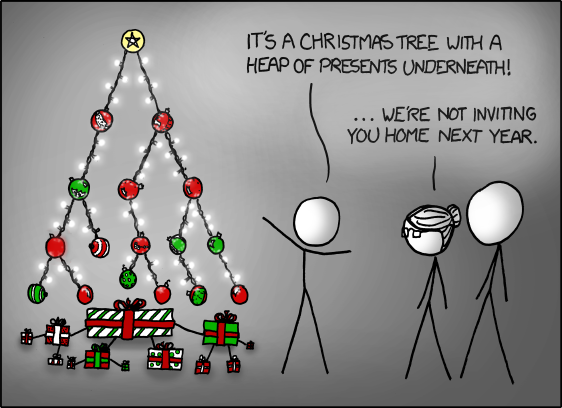
\includegraphics[width=.45\textwidth]{../Images/xkcd-tree.png}
			\caption{XKCD: "\textit{Tree}" \cite{xkcd-tree}}
		\end{figure}
		
		\columnbreak
		
		\null \vfill
		
		Merkle trees are secured data structures whose operations can be used to prove/verify membership of a node in $\mathcal{O}(\log(n))$ hashes.
		%Shrinking public keys. \cite{boneh2020graduate}
		
		\vfill \null
	\end{multicols}
\end{frame}


\section{Operations}

\begin{frame}{Proving Membership (\textit{singular})}
	
	\begin{figure}
		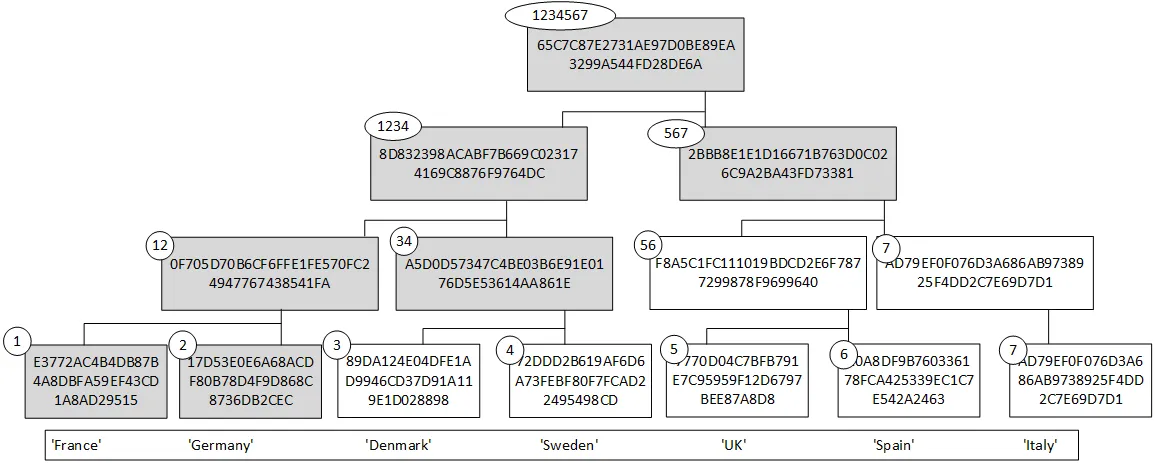
\includegraphics[width=.8\textwidth]{../Images/merkle-example.png}
		\caption{Show Germany exist in the tree \cite{buchannen_2022}}
		% The reason we only need nodes 1, 34 and 567, is that we can regenerate Node 12 and Node 1234 from these values. Bitcoin, for example, uses this method in order to check the validity of a transaction within the block. We can then add our transactions into a Merkle Tree, and produce a root hash. Within the block we can then add the root hash of the previous block and the root hash of the next block, and thus interlock the blocks into a chain:
		
	\end{figure}
\end{frame}

\begin{frame}{Proving Membership (\textit{multiple})}
	
	\begin{figure}
		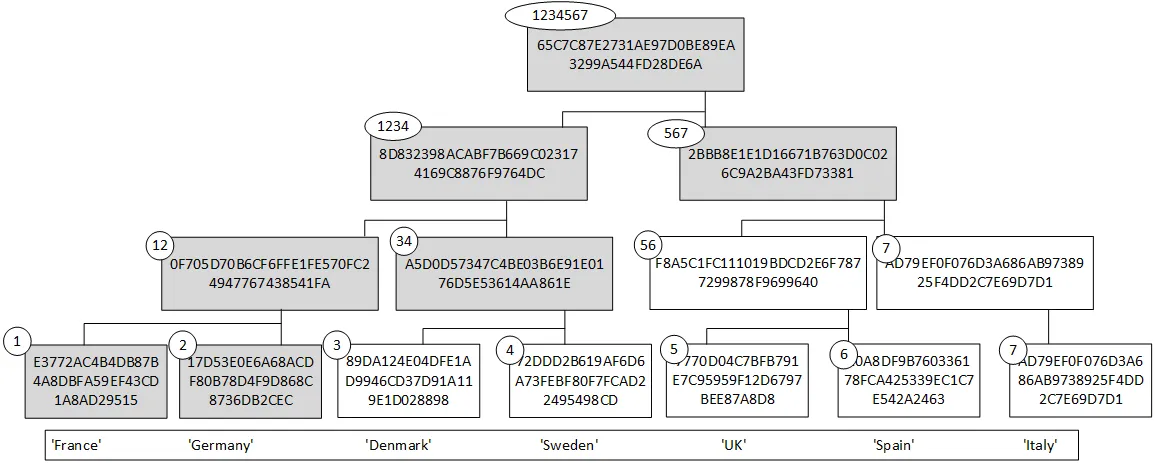
\includegraphics[width=.8\textwidth]{../Images/merkle-example.png}
		\caption{Show Germany \textbf{and} France exist in the tree \cite{buchannen_2022}}
		% The reason we only need nodes 1, 34 and 567, is that we can regenerate Node 12 and Node 1234 from these values. Bitcoin, for example, uses this method in order to check the validity of a transaction within the block. We can then add our transactions into a Merkle Tree, and produce a root hash. Within the block we can then add the root hash of the previous block and the root hash of the next block, and thus interlock the blocks into a chain:
		
	\end{figure}
\end{frame}


\begin{frame}{Joining trees}
% This is key for understanding attacks

\begin{figure}
	See blackboard
	\caption{ Create a new root node and connect trees $A$ and $B$  \cite{boneh2020graduate}}
	% This is innefective if it is a sorted tree
\end{figure}
\end{frame}


\begin{frame}{Equality}
	% This is key for understanding attacks
	
	\begin{figure}
		See blackboard
		\caption{Show trees $A$ and $B$ are equal.}
	\end{figure}
\end{frame}



\section{Security}

% We next define security. We say that an adversary defeats the scheme if it can output a hash value y ∈ Y and then fool the verifier into accepting two different elements x and x 0 in X at some position i.

\begin{frame}{Is it a secure authenticated data structure}
	\begin{quote}
		We next define security. We say that an adversary defeats the scheme if it can output a hash

	\end{quote}

	
	\textbf{We assume the underlying hash function h is collision resistant.}
\end{frame}

% . The Merkle hash tree scheme is a secure authenticated data structure scheme, assuming the underlying hash function h is collision resistan

\begin{frame}{Authenticated data structure scheme syntax}
	An authenticated data structure scheme $\mathcal{D} = (H, P, V )$ defined over $(\mathcal{X}^{n}, \mathcal{Y})$
	is a tuple of three efficient deterministic algorithms:
	\begin{itemize}
		\item $H$ is an algorithm that is invoked as $y \leftarrow H(T)$, where $T := (x_1,\ldots , x_n) \in \mathcal{X}^n$ and $y \in \mathcal{Y}$.
		\item $P$ is an algorithm that is invoked as $\pi \leftarrow P(i, x, T)$, where $x \in \mathcal{X}$ and $1 \leq i \leq n$. The
		algorithm outputs a proof $\pi$ that $x = x_i$, where $T := (x_1, \ldots , x_n)$.
		\item $V$ is an algorithm that is invoked as $V (i, x, y, \pi)$ and outputs accept or reject.
		\item We require that for all $T := (x_1,\ldots , x_n) \in \mathcal{X}^n$, and all $1 \leq i \leq n$, we have that
		$$
		V(i, x_i	, H(T), P(i, x_i, T))  = \mathrm{accept}
		$$
	\end{itemize}
\end{frame}

\begin{frame}{Attack Game}
	For Merkle tree $D = (H, P, V )$ defined over $(\mathcal{X}^{n}, \mathcal{Y})$, and a given adversary $\mathcal{A}$: 
	
	\begin{quote}
		The adversary $A$ outputs a $y \in \mathcal{Y}$, a position $i \in \{1, \ldots , n\}$, and two pairs $(x, \pi)$ and $(x', \pi')$ where $x, x' \in \mathcal{X}$.
	\end{quote}

$\mathcal{A}$ wins the game if $x \neq x'$ and $V(i, x, y, \pi)=V(i, x', y, \pi')=$accept. Define $\mathcal{A}$'s advantage with respect to $\mathcal{D}$, denoted $\mathrm{ADSadv}[\mathcal{A}, \mathcal{D}]$, as the probability that $\mathcal{A}$ wins the game. 
\end{frame}

\begin{frame}{Merkle hash tree scheme is a Secure Authenticated Data Structure Scheme}
	
	\begin{quote}The Merkle hash tree scheme is a secure authenticated data structure scheme,
		assuming the underlying hash function $h$ is collision resistant.  
	\end{quote}
	
\end{frame}



\section{Implementations}

\begin{frame}{Lessons from Bitcoin}
	\begin{multicols}{2}
		\begin{figure}
			
\includegraphics[width=.45\textwidth]{../Images/xkcd-bitcoin.png}
			\caption{XKCD: "\textit{2010 and 2020}" \cite{xkcd-bitcoin}}
		\end{figure}
		
		\columnbreak
		
		\null \vfill
		\begin{itemize}
			\item \st{All cryptocurrencies are Ponzi schemes}
			\item The \textit{chain} is actually collection of root nodes.
			\item Bitcoin incorrectly implemented their merkle trees and it resulted in DOS attacks due to over hashing and duplicate nodes (CVE-2012-2459). 
		\end{itemize}
		\vfill \null
	\end{multicols}
\end{frame}


\begin{frame}{BitTorrent Data Integrity}
	\begin{multicols}{2}
		\begin{figure}
			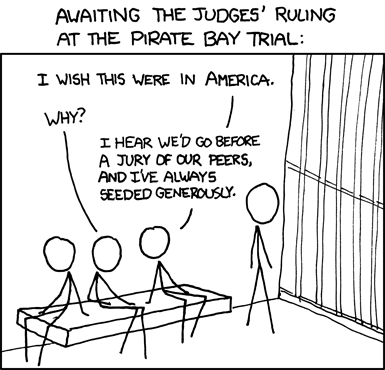
\includegraphics[width=.45\textwidth]{../Images/pirate_bay.png}
			\caption{XKCD: "\textit{Pirate Bay}" \cite{xkcd-pirate-bay}}
		\end{figure}
		
		\columnbreak
		
		\null \vfill
		\begin{itemize}
			\item Finding errors in $\mathcal{O}(\log(n))$!
			\item Only needing to compare nodes below incorrect nodes.
		\end{itemize}
		\vfill \null
	\end{multicols}
\end{frame}

\begin{frame}[allowframebreaks]{References}
\printbibliography
\end{frame}

\end{document}
